\chapter{Implementacija i korisničko sučelje}
		
		
		\section{Korištene tehnologije i alati}
		
			
			 {Organizacija te raspodjela i komunikacija tima odvijala se preko aplikacije \underline{WhatsApp\textsuperscript{1}}. Nadalje UML dijagrami su su napravljeni u alatu \underline{Atash Professional\textsuperscript{2}} te je za upravljanje kodom korišten \underline{Git\textsuperscript{3}}, a cijeli projekt je dostupan na udaljenom repozitoriju u sklopu web aplikacije \underline{GitLab\textsuperscript{4}}}.\\
			
			
			{Pri konstrukciji front end-a korišten je \underline{Microsoft Visual studio code\textsuperscript{5}} - uređivač koda  tvrtke Microsoft. Primarno se koristi kao uređivač koda te sadrži podršku za razvojne operacije kao što su debuggiranje, izvođenje zadataka te verzioniranje. Nadalje pri konstrukciji back end-a korišten  je \underline{IntelliJ IDEA\textsuperscript{6}} integrirano radno okruženje (IDE) tvrtke JetBrains. Primarno se koristi za razvoj softvera napisanog u Javi, Kotlinu te drugim jezicima temeljenim na JVM-u(Java virtual machine) }.\\
			
			{Web aplikacija je napisana koristeći radni okvir \underline{Spring boot\textsuperscript{7}} i jezik \underline{Java\textsuperscript{8}} za izradu back end-a te za izradu front end-a korišten je jezik \underline{JavaScript\textsuperscript{9}}  odnosno njegova biblioteka otvorenog tipa  \underline{React\textsuperscript{10}} održavana od strane tvrtke Meta te neovisni programera. React se najčšće  koristi kao osnova u razvoju web aplikacija. Složene aplikacije u Reactu  zahtijevaju korištenje dodatnih biblioteka za interakciju s API-jem. Radni okvir Spring boot je ekstenzija Spring radnog okvira te eliminira konfiguranciju okvirne ploče potrebne za postavljanje spring aplikacije }.\\
			
			{Baza podataka pisana je u \underline{PostgreSql\textsuperscript{11}} SQL jeziku te je za njeno kreiranje korišten radna okolina \underline{PgAdmin\textsuperscript{12}}. Nadalje aplikacija je podignuta na web pomoću oblaka \underline{Render\textsuperscript{13}}  }.
			
			\noindent\rule{8cm}{0.4pt}
			
			\noindent\textsuperscript{1}https://www.whatsapp.com/ \\
			\textsuperscript{2}https://astah.net/products/astah-professional/ \\
			\textsuperscript{3}https://git-scm.com/ \\
			\textsuperscript{4}https://about.gitlab.com/ \\
			\textsuperscript{5}https://code.visualstudio.com/ \\
			\textsuperscript{6}https://www.jetbrains.com/idea/ \\
			\textsuperscript{7}https://spring.io/projects/spring-boot \\
			\textsuperscript{8}https://www.java.com/en/ \\
			\textsuperscript{9}https://www.javascript.com/ \\
			\textsuperscript{10}https://reactjs.org/ \\
			\textsuperscript{11}https://www.postgresql.org/ \\
			\textsuperscript{12}https://www.pgadmin.org/ \\
			\textsuperscript{13}https://render.com/ \\
			
			
			
			
			\eject 
		
	
		\section{Ispitivanje programskog rješenja}
			
		
	
			
			\subsection{Ispitivanje komponenti}
		
			
			\textbf{Ispitni slučaj 1: Uspješno stvaranje trenera}\\
				\begin{verbatim}
					@Test
					public void testCreatingNewTrainerSuccessfully() throws Exception{
					
						User mockUser = UserGeneratingUtil.createMockUser();
						
						when(userService.newTrainer(mockUser)).thenReturn("success")
						
						mvc.perform(post("/new-trainer").contentType(MediaType.APPLICATION_JSON).content(objectMapper.writeValueAsString(mockUser))).
							andExpect(status().isOk())
							.andExpect(content().string(("success")));
							
				}
				\end{verbatim}\\\\
			
				\textbf{Ispitni slučaj 2: Neuspješno stvaranje trenera}\\\\
				
				\begin{verbatim}
					@Test
					public void testCreatingNewTrainerSuccessfully() throws Exception{
								
									User mockUser = UserGeneratingUtil.createMockUser();
									
									when(userService.newTrainer(mockUser)).thenThrow(new REquest DeniedException("Username: " + mockUser.getUsername() + " is already taken."));
									
									mvc.perform(post("/new-trainer").contentType(MediaType.APPLICATION_JSON).content(objectMapper.writeValueAsBytes(mockUser))).
											andExpect(status().is4xxClientError());
											
											
					}
				\end{verbatim}\\
		
				\begin{figure}[H]
				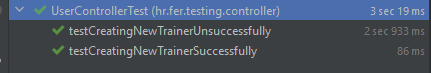
\includegraphics[scale=1]{dijagrami/2.png} %veličina slike u odnosu na originalnu datoteku i pozicija slike
				\centering
				\caption{Rezultati ispitnih slučajeva 1 i 2}
				\label{fig:ispitnislucaj12rez}
			\end{figure}\\\\
		
			
			\textbf{Ispitni slučaj 3: dohvaćanje treninga }\\
			
			\begin{verbatim}
				@Test
				public void testGetAllSessions() {
						
						TrainingSessionEntity mockTs = TrainingGeneratingUtil.createMockSession();
						
						when(trainingSessionRepository.findAll()).thenReturn(List.of(mockTs));
						
						verify(trainingSessionRepository, times(1)).findAll();
						
						Assert.assertEquals(found.size(), 1);
						
				}
			\end{verbatim}\\
			
			
				\begin{figure}[H]
				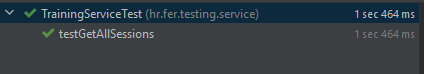
\includegraphics[scale=1]{dijagrami/4.png} %veličina slike u odnosu na originalnu datoteku i pozicija slike
				\centering
				\caption{Rezultat ispitnog slučaja 3}
				\label{fig:ispitnislucaj3rez}
			\end{figure}\\\\
		
		
			\textbf{Ispitni slučaj 4: Prikaz svih ne trenera}\\\\
		
			\begin{verbatim}
				
				@Test
				public void testListingAllNonTrainers() {
					
					User mockUser = UserGeneratingUtil.createMockUser();
					
					UserEntity mockUserEntity = USerEntity.from(mockUser);
					
					when(userRepository.findAll()).thenReturn(List.of(mockUserEntity));
					
					List<UserEntity> found = userService.listAllNonTrainers();
					
					verify(userRepository, times(1)).fidnAll();
					
					Assert.assertEquals(found.size(), 0)
					
			}
			\end{verbatim}\\\\
		
			\textbf{Ispitni slučaj 5: Neuspješno dodavanje novog trenera}\\
			
			\begin{verbatim}
					@Test
					public void testAddingNewTrainerUnsuccessfully() {
						
						User mockUser = UserGeneratingUtil.createMockUser();
						
						UserEntity mockUserEntity = USerEntity.from(mockUser);
						
						when(userRepositroy.findById(mockUser.getUsername())).thenReturn(Optional.of(mockUserEntity));
						
						when(userRepositroy.countByEmail(mockUser.getEmail())).thenReturn(0);
						
						assertThrows(requestDeniedException.class, () -> userService.newTrainer(mockUser));
						
						verfy(userRepository, times(1)).findById(mockUser.getUsername());
						
						verfy(userRepository, times(1)).countByEmail(mockUser.getEmail());
						
					}
			\end{verbatim}\\\\
		
			\textbf{Ispitni slučaj 6: Neuspješno pronalaženja korisnika po ID-u}\\
		
			\begin{verbatim}
				@Test
				public void testFindingUSerByIdUnsuccessfully() {
						
						User mockUser = UserGeneratingUtil.createMockUser();
						
						UserEntity mockUserEntity = USerEntity.from(mockUser);
						
						String mockUsername= "stella";
						
						when(userRepository.findById(mockUsername)).thenReturn(Optional.empty());
						
						UserEntity found = userService.findById(mockUsername);
						
						verfiy(userRepository, times(1)).findById(mockUsername);
						
						Assert.assertEquals(found, null);
							
			}
			\end{verbatim}\\
		
				\begin{figure}[H]
				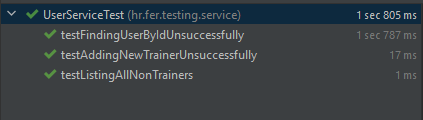
\includegraphics[scale=1]{dijagrami/6.png} %veličina slike u odnosu na originalnu datoteku i pozicija slike
				\centering
				\caption{Rezultati ispitnih slučajeva 4, 5 i 6}
				\label{fig:ispitnislucaj3rez}
			\end{figure}\\\\
			
			\subsection{Ispitivanje sustava}
				
				\textbf{Ispitni slučaj 1: Uspješan pristup kalendaru}
				
				\textbf{Ulaz:}
				\begin{enumerate}
					\item Otvaranje početne stranice web aplikacije
					\item pritisak na gumb "login"
					\item unošenje podataka (korisnik posjeduje postojeći račun)
					\item redirect na stranicu kalendara
				\end{enumerate}
				\textbf{Izlaz:}
				\begin{enumerate}
					\item prikazuje se početna stranica
					\item gumb nas vodi na stranicu login
					\item uspješna prijava
					\item prikaz stranice kalendara
				\end{enumerate}
				\textbf{Rezultati:} {Aplikacija je uspješno izvela sve korake testa. \color{green} Aplikacija je prošla test.}\\\\
				
				
					\begin{figure}[H]
					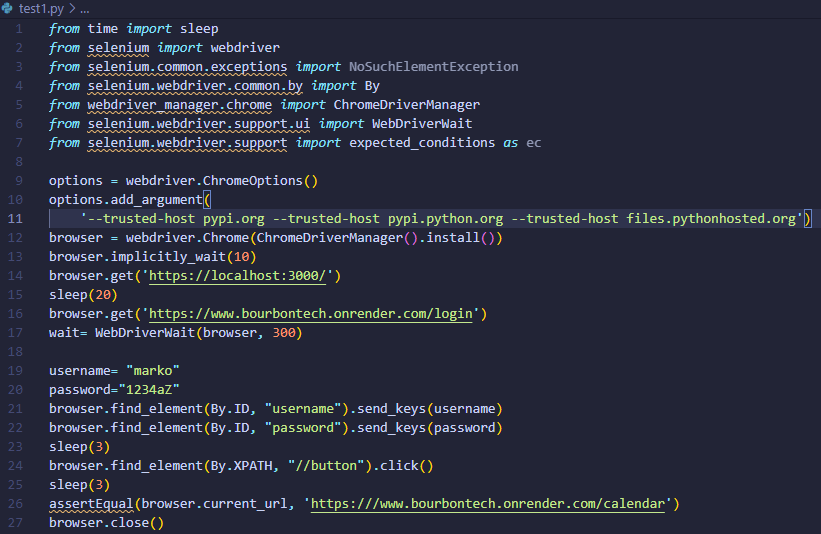
\includegraphics[scale=0.4]{dijagrami/test1.png} %veličina slike u odnosu na originalnu datoteku i pozicija slike
					\centering
					\caption{Izvorni kod ispitnog slučaja 1}
					\label{fig:ispitnislucaj1}
				\end{figure}\\
				
				
					\textbf{Ispitni slučaj 2: Neuspješan pristup kalendaru}
				
				\textbf{Ulaz:}
				\begin{enumerate}
					\item Otvaranje početne stranice web aplikacije
					\item pritisak na gumb "login"
					\item unošenje podataka (korisnik ne posjeduje postojeći račun)
					\item redirect na stranicu neuspjele prijave 
				\end{enumerate}
				\textbf{Izlaz:}
				\begin{enumerate}
					\item prikazuje se početna stranica
					\item gumb nas vodi na stranicu login
					\item uneseni podaci ne odgovaraju ni jednom postojećem računu
					\item prikaz stranice neuspjele prijave
				\end{enumerate}
				\textbf{Rezultati:} {Sve komponente testa su uspješno zadovoljene od strane aplikacije. \color{green} Aplikacija je prošla test.}\\\\
			
					\begin{figure}[H]
					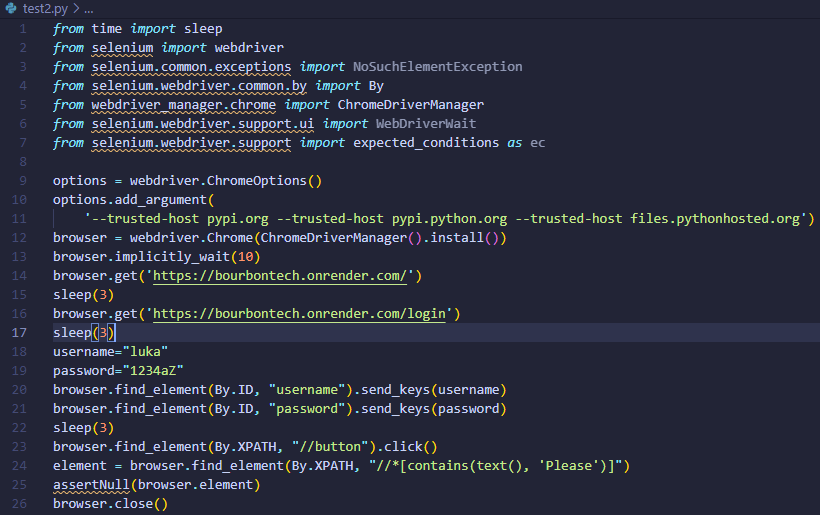
\includegraphics[scale=0.4]{dijagrami/test2.png} %veličina slike u odnosu na originalnu datoteku i pozicija slike
					\centering
					\caption{Izvorni kod ispitnog slučaja 2}
					\label{fig:ispitnislucaj2}
				\end{figure}\\
				
					\textbf{Ispitni slučaj 3: Promjena lozinke}
				
				\textbf{Ulaz:}
				\begin{enumerate}
					\item Otvaranje početne stranice web aplikacije
					\item pritisak na gumb "login"
					\item unošenje podataka (korisnik posjeduje postojeći račun)
					\item redirect na stranicu kalendara
					\item otvaranje stranice profila
					\item pritisak na gumb "change password"
					\item unos stare pa zatim nove lozinke
					\item pritisak na gumb "save"
					\item pritisak na gumb "logout"
					\item pritisak na gumb "login"
					\item prijava s promjenjenim podacima
					\item redirect na stranicu kalendara
				\end{enumerate}
				\textbf{Izlaz:}
				\begin{enumerate}
					\item prikazuje se početna stranica
					\item gumb nas vodi na stranicu login
					\item uspješna prijava
					\item prikaz stranice kalendara
					\item prikaz stranice profila
					\item prikaz forme za promjenu lozinke
					\item nova lozinka spremljena
					\item korisnik odjavljen
					\item gumb nas vodi na stranicu login
					\item uspješna prijava
					\item prikaz stranice kalendara
				\end{enumerate}
				\textbf{Rezultati:} {Aplikacija je pravilno i efikasno izvela zahtjeve testa. \color{green} Aplikacija je prošla test.}\\\\
				
					\begin{figure}[H]
					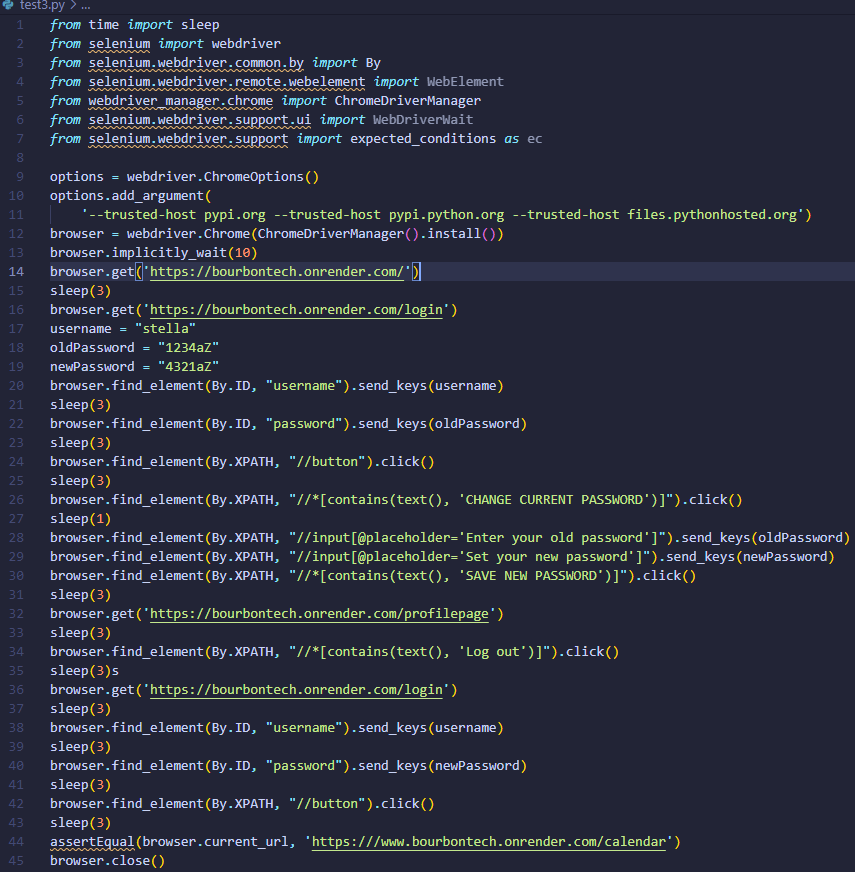
\includegraphics[scale=0.4]{dijagrami/test3.png} %veličina slike u odnosu na originalnu datoteku i pozicija slike
					\centering
					\caption{Izvorni kod ispitnog slučaja 3}
					\label{fig:ispitnislucaj3}
				\end{figure}\\
				
				
				\textbf{Ispitni slučaj 4: Rezervacija treninga}
				
				\textbf{Ulaz:}
				\begin{enumerate}
					\item Otvaranje početne stranice web aplikacije
					\item pritisak na gumb "login"
					\item unošenje podataka (korisnik posjeduje postojeći račun)
					\item redirect na stranicu kalendara
					\item klik na gumb "reservation"
					
				\end{enumerate}
				\textbf{Izlaz:}
				\begin{enumerate}
					\item prikazuje se početna stranica
					\item gumb nas vodi na stranicu login
					\item uspješna prijava
					\item prikaz stranice kalendara
					\item smanjivanje fonda sati za jedan
				\end{enumerate}
				\textbf{Rezultati:} {Testiranje aplikacije je završilo uspješno. \color{green} Aplikacija je prošla test.}\\\\
				
				
					\begin{figure}[H]
					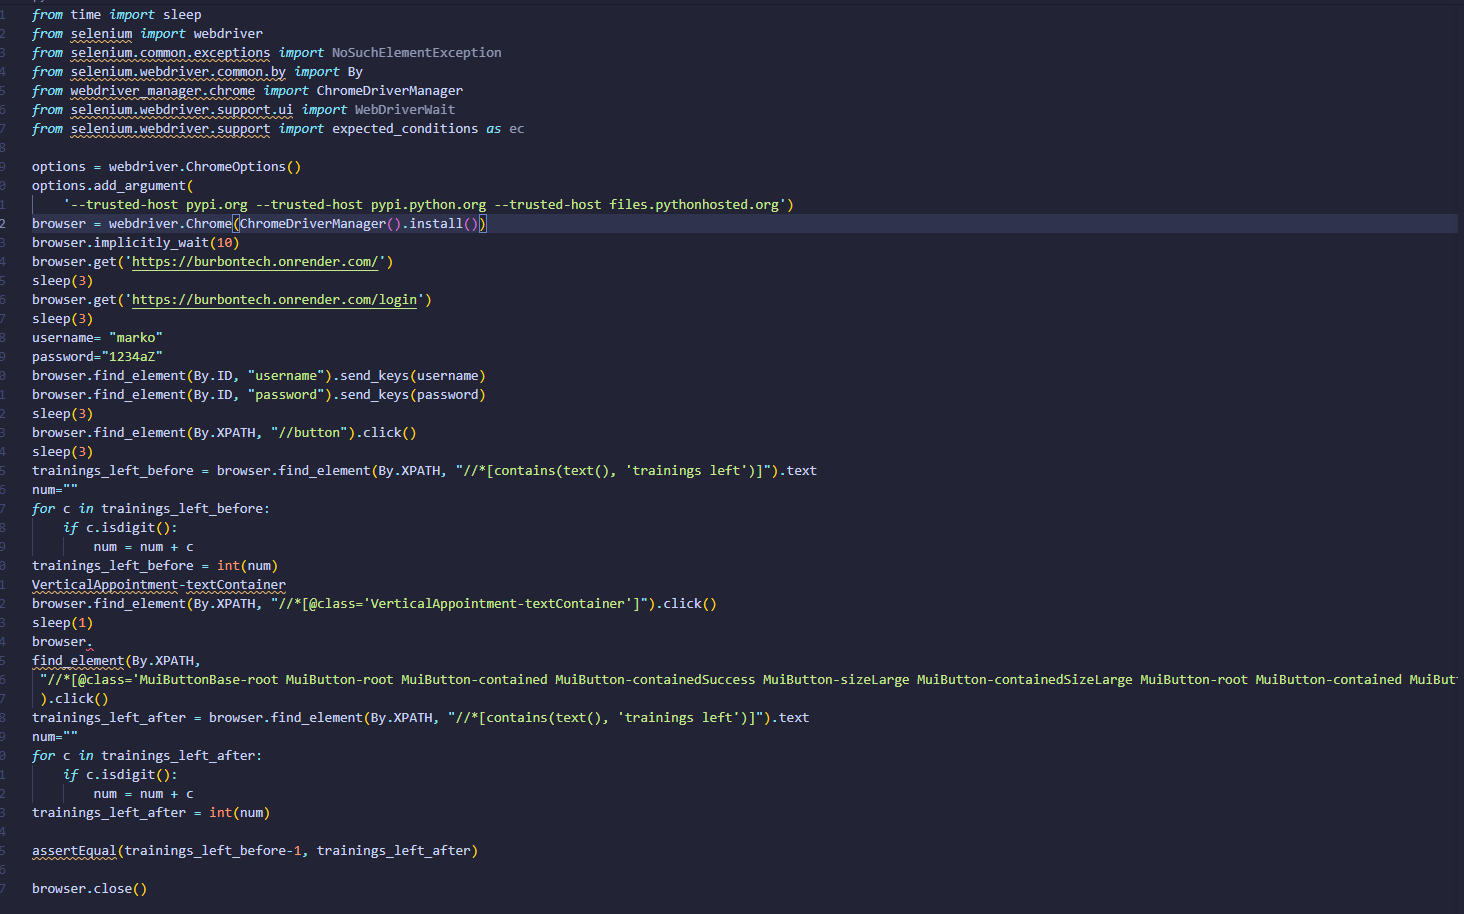
\includegraphics[scale=0.4]{dijagrami/test4.png} %veličina slike u odnosu na originalnu datoteku i pozicija slike
					\centering
					\caption{Izvorni kod ispitnog slučaja 4}
					\label{fig:ispitnislucaj4}
				\end{figure}\\
		
		\section{Dijagram razmještaja}
			
			{Dijagrami razmještaja su strukturni statički UML dijagrami koji opisuju topologiju sustava i usredotočeni su na odnos sklopovskih i programskih dijelova. Na strani poslužitelja se nalazi web poslužitelj te poslužitelj baze podataka. Dok se na strani klijenta nalazi web preglednik kojim korisnik pristupa aplikaciji. Sustav je koncipiran na arhitekturi "klijent-poslužitelj" te se komunikacija odvija putem HTTP veze}. \\
			
			
			\begin{figure}[H]
				\includegraphics[scale=0.4]{dijagrami/dijagramRazmještaja.png} %veličina slike u odnosu na originalnu datoteku i pozicija slike
				\centering
				\caption{dijagram razmještaja }
				\label{fig:diagramrazmještaja}
			\end{figure}
			
			\eject 
		
		\section{Upute za puštanje u pogon}
		
			
			
			\textbf{Priprema backend-a za deploy na Render}\\
		
			{Po potrebi dodati env. varijable u run konfiguraciju vašeg IDE-a. Zatim dodati Dockerfile uz napomenu da u direktoriju docker postoje dvije verzije, za Maven i Gradel. Nadalje ukoliko se mijenja lokacija DockerFile-a pripaziti na putanju unutra "COPY" naredbi u DockerFile skripti. U application.properties postaviti property server.servlet.context-path na /api kao prefiks svim zahtjevima na backend. }.\\
			
			\noindent\textbf{Priprema frontend-a za deploy na Render}\\
			
			{U package.json potrebno je dodati dependency-e neophodne za deploy to jest primarno http-proxy-middleware, dontev te express. Zatim potrebno je dodati /src/setupProxy.js koji služi kao proxy server za lokalni development (preusmjerava api pozive na localhost:8080) odnosno kada se koristi "react-scripts start" skripta. Nadalje potrebno je dodati app.js u kojem se nalazi express server za produkcijski proxy te poosluživanje frontend-a. Također potrebno je u package.json izmjeniti \begin{verbatim}
					"build": "yarn install && react-scripts build"\end{verbatim}  te dodati \begin{verbatim}
					"start-prod": "node app.js"
				\end{verbatim} }.\\
			
			\noindent\textbf{Deploy}\\
			
			\textbf{Kreiranje baze podataka}\\
				{Potrebno je u Render dashboard-u izvesti sljedeće komande :
				\begin{itemize}
					\item New $\Rightarrow$ PostgreSQL
					\item Postaviti ime baze i opcionalno username za korisnika baze (password je automatski generiran)
					\item Region Frankfurt
					\item Create Database
					\item Free plan baza podataka ima max pohranu od 1GB 
			\end{itemize}}.\\
			\textbf{Kreiranje backend-a}\\
				{Potrebno je u Render dasboard-u izvesti sljedeće komande :
					\begin{itemize}
						\item New $\Rightarrow$ Web Service
						\item Povezati Gitlab racun, nakon čega su za odaabir dostupni svi projekti na koje imate prava pristupa
						\item Stisnuti connect pored odgovarajućeg projekta
						\item Postaviti ime za servis(postaje dio web adrese)
						\item Rot directory postaviti na progi-be
						\item Environment Docker
						\item Region Frankfurt
						\item Na dnu proširiti advanced
						\item Dodati potrebne environment varijable te kopirati vrijednosti iz postavki baze podataka na Renderu. 
						\item Ako je dodan Spring Boot Actuator postaviti /api/actuator/health kao Healt Check Path
						\item Postaviti putanju za DOckerfile ovisno o pacage menageru 
						\item Stisnuti Create Web Service
				\end{itemize}}
			\textbf{Kreiranje frontend-a}\\
				{Potrebno je u Render dashboard-u izvesti sljedeće komande :
					\begin{itemize}
						\item New $\Rightarrow$ Web Service
						\item  Povezati Gitlab racun, nakon čega su za odaabir dostupni svi projekti na koje imate prava pristupa
						\item Stisnuti connect pored odgovarajućeg projekta
						\item Postaviti ime za servis(postaje dio web adrese)
						\item Rot directory postaviti na progi-fe
						\item Environment Node
						\item Region Frankfurt
						\item Build command postaviti na yarn build, a Start Command yarn start-prod
						\item Na dnu proširiti advanced
						\item Dodati potrebne environment varijable -API\_BASE\_URL postaviti na adresu deployanog backend-a aplikacije dostupne na Render dashboardu
						\item Stisnuti Create Web Service
				\end{itemize}}.\\
			
			
			\eject 